\section{The reviewed Study}
\label{sec:summary}

The general topic of the reviewed paper is to conduct an SMS over the topic
of ``Microservices in DevOps''. We should take into consideration, that the context
is specifically set to ``DevOps''. Recent years and recent developments
raised the attention to the topic significantly. Furthermore, at the
time of writing of the paper, no comprehensive review of the research was
available. The study asks several research questions (RQs) and conducts
a systematic mapping study (SMS) upon two defined search queries. Then,
after screening and analyzing the results, the authors created a mapping
to certain categories and several problems and their solutions.
After a presentation of the results, Waseem et al. provide a broad discussion of the found
results shows some differences between the theory and effective
results \cite{waseem:SMSMSADevOps}.

\subsection{Motivation}

The purpose of the reviewed paper is to create an SMS to understand how
Microservice Architecture (MSA) is used in conjunction with DevOps.
Furthermore the objective is to identify, analyze and categorize the
existing literature and research around the given topic.
In addition to that, problems and their corresponding solutions - if any - should
be identified. The contribution of the paper to the
academia is a classification of the research, a classification of problems
and their solution, a list of identified research challenges, a classification of
used tools and a list of formal or informal description
tools for MSA \cite{waseem:SMSMSADevOps}.

\subsection{Methodology}

With the goal to not limit the results of such an empirical software engineering method
to one specific research question, the authors conducted an SMS instead of an SLR,
which provides insight and secondary data for a particular question.
The SMS contained three essential steps \cite{waseem:SMSMSADevOps}:

\begin{enumerate}
    \item Planning the mapping study
    \item Collection and analyzing the data
    \item Mapping and documenting the results
\end{enumerate}

The authors built the conducted SMS upon the guidelines proposed by Kai Petersen \cite{petersen:SMS}.

\subsection{Research Questions}

Ten different RQs in four categories were derived
according to the goal of the paper \cite{waseem:SMSMSADevOps}:

~\\
\begin{table}[H]
    \begin{tabularx}{\columnwidth} {
            | m{0.12\columnwidth}
            | X |}
        \hline
        \multicolumn{2}{ | X | }{
            \textbf{Category 1: Demography, classification,
            and mapping of research}
        }                                                  \\
        \hline
        RQ1.1
         &
        What is the frequency and type of published research
        on MSA in DevOps?                                  \\
        \hline
        RQ1.2
         &
        What are the existing research themes on MSA in
        DevOps and how can they be classified and mapped?  \\
        \hline
        \multicolumn{2}{ | X | }{
            \textbf{Category 2: Problems, solutions, and challenges}
        }                                                  \\
        \hline
        RQ2.1
         &
        What problems have been reported when implementing
        MSA in DevOps?                                     \\
        \hline
        RQ2.2
         &
        What solutions have been employed to address the
        problems?                                          \\
        \hline
        RQ2.3
         &
        What challenges have been reported when
        implementing MSA in DevOps?                        \\
        \hline
        \multicolumn{2}{ | X | }{
            \textbf{Category 3: MSA description methods, patterns,
            and quality attributes}
        }                                                  \\
        \hline
        RQ3.1
         &
        What methods are used to describe MSA in DevOps?   \\
        \hline
        RQ3.2
         &
        What MSA design patterns are used in DevOps?       \\
        \hline
        RQ3.3
         &
        What quality attributes are affected when employing
        MSA in DevOps?                                     \\
        \hline
        \multicolumn{2}{ | X | }{
            \textbf{Category 4: Tool support and application domains}
        }                                                  \\
        \hline
        RQ4.1
         &
        What tools are available to support MSA in DevOps? \\
        \hline
        RQ4.2
         &
        What are the application domains that employ MSA in
        DevOps?                                            \\
        \hline
    \end{tabularx}
    \caption{Given research questions}
    \label{tbl:RQs}
\end{table}

\autoref{tbl:RQs} shows the research questions that the authors
tried to solve with the systematic mapping study.

\subsection{Search}

To collect data, Waseem et al. used a two-phase-search. The first search was applied
to the selected databases with the created search-query. The secondary
search used a technique called ``snowballing''. ``Forward snowballing''
includes studies that cite the found studies, while ``backward snowballing''
follows the references of the found research material \cite{wohlin:Snowballing}.

The study limited the search to peer-reviewed studies from January 2009 until
July 2018. They chose this particular starting point because the term ``DevOps''
was introduced in the year 2009 \cite{waseem:SMSMSADevOps}.

Since MSA has multiple synonyms and can be in context with DevOps or without
the said context, the following two search-strings were compiled \cite{waseem:SMSMSADevOps}:

\begin{enumerate}
    \item \texttt{((microservi* OR micro-servi*)
              AND (architect* OR design OR structur*) AND DevOps)}
    \item \texttt{(microservice AND DevOps)}
\end{enumerate}

It is worth noting that the contextual part ``DevOps'' is not optional nor is
it a construct like ``microservi*''. This limits the results to publications
that must contain the term ``DevOps'' in their title.

The search was executed on the following seven databases \cite{waseem:SMSMSADevOps}:

\begin{itemize}
    \item ACM Digital Library (\url{https://dl.acm.org})
    \item Springer Link (\url{https://link.springer.com})
    \item Wiley InterScience (\url{https://onlinelibrary.wiley.com})
    \item EI Compendex (\url{https://www.engineeringvillage.com})
    \item IEEE Xplore (\url{https://ieeexplore.ieee.org})
    \item Science Direct (\url{https://www.sciencedirect.com})
    \item ISI Web of Science (\url{https://webofknowledge.com})
\end{itemize}

The search for the first four databases (ACM until EI Compendex) was executed
on the title of the publication, as well as their abstract. The other three
databases also included ``keywords'' in the search targets.

The execution of the provided search queries on the given databases
yielded a total of 494 studies. After the initial search, the authors
screened and categorized the found studies into relevant and irrelevant
publications. Of the original 494 studies, only 285 were flagged as ``relevant''.
\smsAuthors then analyzed the studies according to six generic screening and one specific
screening aspect. An example of such a generic aspect is: ``Is the study written in English?''.
Whereas the specific one states: ``Does the study present problems, solutions, challenges,
description methods, patterns, QAs, and tools in the context of
MSA and DevOps combination?'' \cite{waseem:SMSMSADevOps}.

After the screening, 117 remained flagged as relevant.
Those 117 studies were fully read and scored by the authors according to inclusion and
exclusion criteria. At the point when the authors read and assessed all 117 studies,
only 45 studies remained in the relevant category.

In addition to the conducted search, the snowballing technique
yielded additional two studies that were included in the study.
The authors compared the results of the snowball with the found results of the
initial search and then the same practices were applied to those
publications found with the snowball search.

After the search, a total count of 47 different studies remained
relevant for the SMS \cite{waseem:SMSMSADevOps}.

\subsection{Results}

After the conducted search and the thorough analytical readings and classification
of the 47 studies, the collected results were separated in multiple sections
to answer the RQs given in \autoref{tbl:RQs}:

\begin{itemize}
    \item Demography and classification
    \item Problems, solutions and challenges
    \item Description methods, patterns and quality attributes
    \item Tools and application domain
\end{itemize}

The following sections will summarize the found results to
the specific research questions.

\subsubsection{Demography and Classification}

This subsection shall tackle RQ1.1 and RQ1.2 from \autoref{tbl:RQs}.

The conducted search had a year span from 2009 to 2018 \cite{waseem:SMSMSADevOps}.
Despite the broad search parameters of nearly considering a decade worth
of publications, all of the relevant publications were published between
2015 and 2018. The following graph (\autoref{fig:publicationActivity})
should give some insight into the yearly publication rate and the type of publication:

\begin{figure}[h]
    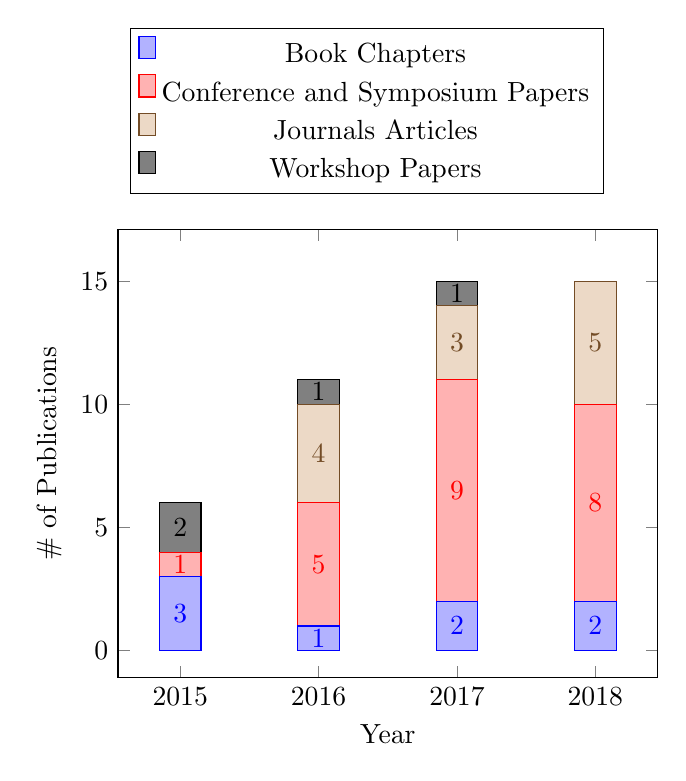
\begin{tikzpicture}
        \begin{axis}[
                ybar stacked,
                bar width=15pt,
                nodes near coords,
                enlargelimits=0.15,
                legend style={
                        cells={align=left},
                        at={(0.9,1.45)}
                    },
                ylabel={\# of Publications},
                xlabel={Year},
                symbolic x coords={2015, 2016, 2017, 2018},
                xtick=data,
                x tick label style={anchor=north},
            ]
            \addplot+[ybar] plot coordinates {
                    (2015,3)
                    (2016,1)
                    (2017,2)
                    (2018,2)
                };
            \addplot+[ybar] plot coordinates {
                    (2015,1)
                    (2016,5)
                    (2017,9)
                    (2018,8)
                };
            \addplot+[ybar] plot coordinates {
                    (2015,0)
                    (2016,4)
                    (2017,3)
                    (2018,5)
                };
            \addplot+[ybar] plot coordinates {
                    (2015,2)
                    (2016,1)
                    (2017,1)
                    (2018,0)
                };
            \legend{
                \strut Book Chapters,
                \strut Conference and Symposium Papers,
                \strut Journals Articles,
                \strut Workshop Papers
            }
        \end{axis}
    \end{tikzpicture}
    \caption{Publication activity}
    \label{fig:publicationActivity}
\end{figure}

The distribution of publications over the years gives a detailed intuition
about the general interest of researchers in the specified topic. As seen
in the diagram above, the topic grew more important over the years 2017 and
2018. Since the first publications in 2015 there is an upward trend to
the number of publications \cite{waseem:SMSMSADevOps}.

As for the publication types, over those four years, 23 studies
were published in conference proceedings, twelve in journals, eight in book chapters
and merely four as workshop papers \cite{waseem:SMSMSADevOps}.

The 47 considered papers were all published in 41 venues. The venues
themselves can be divided into four different categories. 17 of the 41
venues count towards the topic \textbf{Internet, Cloud, and Services Computing}.
Another 16 are categorized as \textbf{Software Engineering} venues. The remaining
eight are split evenly between \textbf{Telecommunications and Networks} with four venues
and \textbf{Multi-Disciplinary computing} also with four venues \cite{waseem:SMSMSADevOps}.

As for RQ1.2, the result shows, that top two subtopics of the publications
are \textit{Approaches} (13 studies) and \textit{Tools} (twelve studies).
The least discussed topic, with only four studies, is \textit{Monitoring}
of microservices \cite{waseem:SMSMSADevOps}.

\subsubsection{Problems, Solutions, and Challenges}

During the SMS, with the aid of a thematic analysis on the
extracted data, a total of 24 problems could be identified.
There exist several problems that could not be mapped with a documented
solution so they represent challenges that need further investigation
to provide the community with possibilities to resolve the problem.

The following lists should give a brief overview of the identified
problems with an associated problem category. Inside the problem domain,
the problems are not specifically ordered \cite{waseem:SMSMSADevOps}.

\textbf{Requirements of MSA-based Systems in DevOps}
\begin{itemize}
    \item Performance Issue due to Lack of Dedicated Access
          to the Host's Hardware
    \item Empowering Developers through Intelligent Software
    \item Performance Overhead due to Fine Grain Decomposition
    \item Scaling MSA-based Systems
\end{itemize}

\textbf{Design of MSA-based Systems in DevOps}
\begin{itemize}
    \item Security and Privacy Across Cloud-Native Applications
    \item Providing Flexible Authentication to Each DevOps Team
    \item Application Decomposition into Microservices
    \item Reducing the Uncertainty in MSA
\end{itemize}

\textbf{Implementation of MSA-based Systems in DevOps}
\begin{itemize}
    \item Managing and Migration Legacy Databases
    \item Modification and Integration of New Functionality in Existing
          Microservices
    \item Operational and Configuration Complexity
\end{itemize}

\textbf{Testing of MSA-based Systems in DevOps}
\begin{itemize}
    \item Testing of MSA-based Systems in DevOps
\end{itemize}

\textbf{Deployment of MSA-based Systems in DevOps}
\begin{itemize}
    \item Frequent Deployment in Different Environments
    \item Complexity in the Dynamic Deployment
    \item Deployment of MSA-based SaaS at Fine Granular Level
    \item Automatic Optimal Deployment of MSA-based Systems
\end{itemize}

\textbf{Monitoring of MSA-based Systems in DevOps}
\begin{itemize}
    \item Logging and Post-Deployment Monitoring
    \item Monitoring and Execution of the Adaptive Actions
    \item Establishing and Maintaining Monitoring Infrastructure
    \item Monitoring Microservices at Run Time
\end{itemize}

\textbf{Organizational Problems}
\begin{itemize}
    \item Introducing DevOps and MSA Culture
    \item People Resistance to Adopting DevOps and Microservices
    \item Less Familiarity with Implementing DevOps
\end{itemize}

\textbf{Resource Management Problems}
\begin{itemize}
    \item Resource management for Development, Deployment,
          and Maintenance of the Cloud-Native Systems
\end{itemize}

For each of the problems in the shown lists, the considered publications
provide at least one solution which can be viewed in ``Figure 6''
of the reviewed study. In general, a proposed idea to tackle multiple
of the problems is to try not to decompose microservice applications
too fine-grain \cite{waseem:SMSMSADevOps}. As for the general problem
category ``designing MSA based systems'', multiple solutions are provided.
A variety of architectures are promoted and evaluated \cite{waseem:SMSMSADevOps}.

To implement MSA based systems in a DevOps context, many studies suggest
automated pipelines as well as automatic testing libraries. For communicating
with other services, agnostic (i.e. independent and non-proprietary)
technologies should be used (like REST over HTTP)
to negate the need of knowledge of a specific programming language
\cite{waseem:SMSMSADevOps}.

Testing MSA based applications and systems should, according to the considered
papers, be tackled with the given testing strategies that are in place
right now. Which means ``unit testing'', ``integration testing'',
``regression testing'', among others \cite{waseem:SMSMSADevOps}.

The topic of deploying MSA based systems is covered mostly by containerization
and tools like ``Docker Compose'' and ``Kubernetes'' \cite{waseem:SMSMSADevOps}.

Monitoring is proposed to be addressed with frameworks like
``Unicorn''\footnote{\url{https://www.technative.io/unicorn-framework-the-rise-of-devops-as-a-service/}}
and patter-based approaches like Omnia\footnote{Elaborated in \cite{miglerina:Omnia}}.
The general goal should be, that each team that owns the microservice should be enabled
to monitor their responsibilities \cite{waseem:SMSMSADevOps}.

Problems that relate to culture, people, cost, and other organizational
topics are proposed to be dealt with guidelines for adopting to
new structures in organizations. Cross-functional teams should be introduced
and they should receive training to spread the acceptance of the
new technology \cite{waseem:SMSMSADevOps}.

As for the topic of resource management problems, some considered
studies proclaim to use virtualized or containerized approaches
and well established platforms to share the workspace among
the developers \cite{waseem:SMSMSADevOps}.

~\\
On the contrary, three challenges were identified which
remained unresolved by the papers that were accounted for \cite{waseem:SMSMSADevOps}:

\begin{itemize}
    \item Performance issues due to frequent communication
    \item Providing security at runtime
    \item Generating runtime architectural models
\end{itemize}

Performance issues can emerge when using too fine-grain microservices
or when using synchronous communication channels to other services.

Studies found that security tends to be neglected in general which leads
to severe vulnerabilities at runtime for microservice based architectures.

Generating models for MSA systems at runtime seems to be an unresearched
topic but could be needed to help with decision-making processes in
adaptive system development.

\subsubsection{MSA descriptions methods, patterns, and quality attributes}

The topic of the third category of RQs orbits around descriptive methods
of MSA systems. What methods and patterns are used and which
quality attributes they should suffice. The regarded studies provided
different patterns and methodologies to describe their architectures
and systems. To summarize the found description methods, five categories
emerged \cite{waseem:SMSMSADevOps}:

\begin{enumerate}
    \item Boxes and Lines (without any "framework")
    \item Unified Modeling Language (UML)
    \item Formal method (e.g. $\pi$-Calculus or equivalent)
    \item Architecture Description Language (ADL)
    \item Entity Relationship Diagrams (ERD) or Business
          Process Modeling Notations (BPMN)
\end{enumerate}

Out of the 47 studies, 46 used some kind of description.
The distribution is shown in \autoref{fig:Distribution}.

\begin{figure}[ht]
    \begin{tikzpicture}
        \pie [rotate = 180]{
            69.5/Boxes and Lines,
            13/UML,
            8/Formal method,
            6.5/ADL,
            3/Others
        }
    \end{tikzpicture}
    \caption{Distribution of descriptive methods}
    \label{fig:Distribution}
\end{figure}

To achieve microservice architecture in complex systems, a multitude of
patterns are proposed over all studies. The SMS identified 38 different design
patterns across all regarded papers. \smsAuthors organized the mentioned
patterns in the following three categories \cite{waseem:SMSMSADevOps}:

\begin{enumerate}
    \item Circuit Breaker (five studies)
    \item ``Migration pattern'' (four studies) \cite{waseem:SMSMSADevOps}
          \footnote{The reviewed SMS does not disclose which specific patterns or languages
              refers to here}
    \item Observer pattern (two studies)
\end{enumerate}

The circuit breaker pattern enables an MSA-based system to ``fail fast''.
The pattern aims to prevent parts of a microservice architecture to cascade
a failure beyond its own boundaries, which in turn could lead to a total
system failure. Instead of waiting for unresponsive services, after some time
the circuit breaker assumes the worst and deals with the fact that the
work unit has become unavailable \cite{montesi:CircuitBreakers}.

The observer pattern is a software design pattern in which some object (i.e. the ``subject'')
maintains a list of observers. Whenever the subject changes its state, it automatically
notifies all observers \cite{gof:DesignPatterns}.

Regarding affected quality attributes when using MSA in the DevOps context,
the presence of said quality attributes (QA) was confirmed by the SMS.
The QAs were split into two sections, one for positively influenced QAs when
using microservices and one for the negative influenced ones \cite{waseem:SMSMSADevOps}.

\textbf{Positive}
The studies listed the following QAs as being positively influenced:
\begin{itemize}
    \item Deployability (42 studies)
    \item Scalability (32 studies)
    \item Performance (26 studies)
    \item Maintainability (27 studies)
    \item Monitoring (23 studies)
    \item Testability (22 studies)
    \item Flexibility (20 studies)
    \item Availability (19 studies)
    \item Efficiency (19 studies)
    \item Security (ten studies)
    \item Portability (six studies)
    \item Compatibility (five studies)
    \item Modifiability (five studies)
    \item Usability (one study)
\end{itemize}

\textbf{Negative}
Some studies listed the following QAs as being negatively influenced:
\begin{itemize}
    \item Security (eleven studies)
    \item Performance (nine studies)
    \item Scalability (two studies)
    \item Reliability (two studies)
    \item Availability (one study)
    \item Compatibility (one study)
    \item Maintainability (one study)
    \item Modifiability (one study)
    \item Usability (one study)
\end{itemize}

To have a view from positively mentioned against negatively mentioned,
consider the following chart which is adapted from the data in the study:

\begin{figure}[H]
    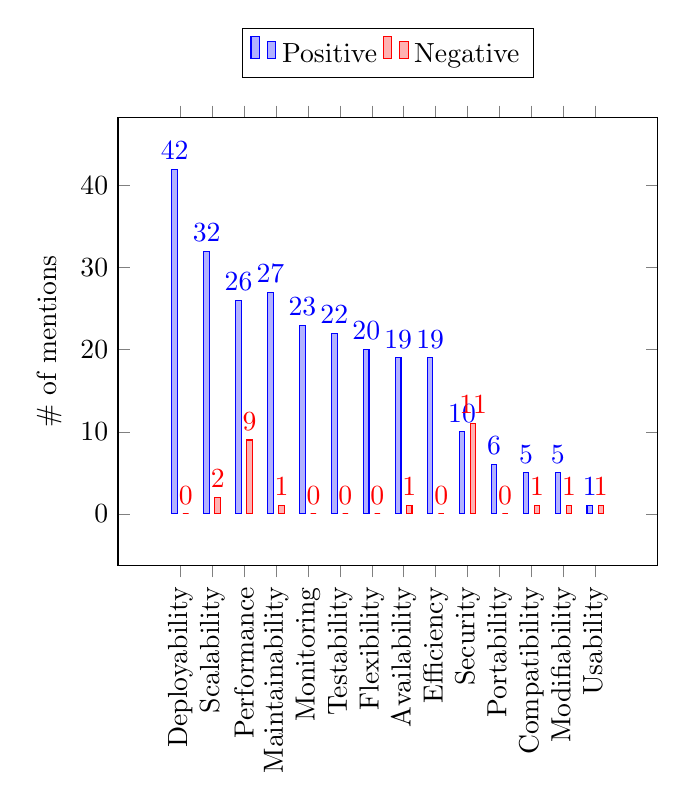
\begin{tikzpicture}
        \begin{axis}[
                ybar,
                bar width=2pt,
                enlargelimits=0.15,
                legend style={
                        at={(0.5,1.2)},
                        anchor=north,legend columns=-1
                    },
                ylabel={\# of mentions},
                symbolic x coords={
                        Deployability,
                        Scalability,
                        Performance,
                        Maintainability,
                        Monitoring,
                        Testability,
                        Flexibility,
                        Availability,
                        Efficiency,
                        Security,
                        Portability,
                        Compatibility,
                        Modifiability,
                        Usability
                    },
                xtick=data,
                x tick label style={rotate=90,anchor=east},
                nodes near coords,
                nodes near coords align={vertical},
            ]
            \addplot coordinates {
                    (Deployability,42)
                    (Scalability,32)
                    (Performance,26)
                    (Maintainability,27)
                    (Monitoring,23)
                    (Testability,22)
                    (Flexibility,20)
                    (Availability,19)
                    (Efficiency,19)
                    (Security,10)
                    (Portability,6)
                    (Compatibility,5)
                    (Modifiability,5)
                    (Usability,1)
                };
            \addplot coordinates {
                    (Deployability,0)
                    (Scalability,2)
                    (Performance,9)
                    (Maintainability,1)
                    (Monitoring,0)
                    (Testability,0)
                    (Flexibility,0)
                    (Availability,1)
                    (Efficiency,0)
                    (Security,11)
                    (Portability,0)
                    (Compatibility,1)
                    (Modifiability,1)
                    (Usability,1)
                };
            \legend{
                \strut Positive,
                \strut Negative
            }
        \end{axis}
    \end{tikzpicture}
    \caption{Influenced Quality Attributes}
\end{figure}

\subsubsection{Tool support and application domains}

The fourth category of research questions regards tooling support
and given application domains. The SMS identified 50 different tools and
11 application domains.

The various tools can be seen in Fig. 7 in the SMS \cite{waseem:SMSMSADevOps}.
The authors categorized them in the following list:

\begin{itemize}
    \item Security Services and Tools (14 tools)
    \item Monitoring Tools (eleven tools)
    \item Continuous Integration Tools (seven tools)
    \item Testing Tools (six tools)
    \item Configuration Management Tools (five tools)
    \item Build Tools (five tools)
    \item Version Control Tools (two tools)
\end{itemize}

The last RQ that is to be answered, is which application domains
exploit the combination of MSA with DevOps. The SMS pinpointed nine
application domains with analyzation of the systems and topics
in the regarded studies. \smsAuthors identified the following
application domains in their study \cite{waseem:SMSMSADevOps}:

\begin{itemize}
    \item Not Mentioned (15 studies) \footnote{Those 15 studies
              did not mention any specific information regarding application
              domains}
    \item Software Development Tools and Framework (eleven studies)
    \item Telecommunication (six studies)
    \item Mobile Software (four studies)
    \item E-Commerce system (three studies)
    \item Embedded system (three studies)
    \item Financial software (three studies)
    \item Healthcare software (one study)
    \item Webserver (one study)
    \item Distributed system (one study)
    \item Autonomic Management System (one study)
    \item Betting and Gaming (one study)
    \item Web Blog (one study)
    \item eServices Developments (one study)
    \item Container Management System (one study)
    \item Content Management (one study)
    \item Software for non-profit (one study)
\end{itemize}

As this list shows, beside studies that did not mention their concrete
application domain, ``Software Development Tools and Framework''
has gained the most attention of all identified application domains
in the study \cite{waseem:SMSMSADevOps}.

\subsection{Discussion}

The following sections summarizes the ``Discussion'' of the SMS. The study
analyzed the found results and explained certain trends.

\subsubsection{Research Status and Themes}

The limitation of the search to peer-reviewed literature from January 2009 to
July 2018 is based on the ``creation'' of the terms MSA and DevOps.
But the rise of papers and studies followed seven years later, around January 2016.
The study noticed, that 41 papers were published from January 2016 until July 2018
\cite{waseem:SMSMSADevOps}.

As seen in the systematic classification of the research themes, the most recurring
topics are ``Tools'' with 13 studies, ``Approaches'' with twelve studies and
``Development and Deployment'' with twelve studies. This indicates, that the research
is not only centered around new tools, but also regards development life-cycles
as well. On the other hand, there were no publications found that focus on
the topic of ``Requirements Engineering'', be it practices or any other
activities \cite{waseem:SMSMSADevOps}.

\subsubsection{Problems and Solutions}

The given solutions in the regarded publications consist of
design patterns, guidelines, frameworks, etc. For example,
Domain Driven Design (DDD) and Model View Controller (MVC) patterns
are recommended for decomposing an application into a microservice oriented
system. The SMS also states that there are no studies found that
address testing strategies for MSA based systems. As for optimal deployment
of MSA, a very popular solution is the usage of containerization and Kubernetes
\cite{waseem:SMSMSADevOps}.

\subsubsection{Challenges}

A big concern in several papers is performance of such MSA based systems.
The impact can be due to frequent communication between microservices.
Also, poorly engineered architectures can lead to wide spread requests
across the whole system. Also, when containers are used, the hardware underneath
has a high impact on performance. The study shows that Amazon EC2 containers are
worse than applications deployed on Amazon EC2 VMs \cite{waseem:SMSMSADevOps}.

The second topic that gets addressed with high frequency, is security. When just ``translating''
applications to MSA, most of the time, security concerns arise. MSA based systems
create complex access control scenarios without any matured patterns to harden
the systems against attackers \cite{waseem:SMSMSADevOps}.

\subsubsection{Description Methods and MSA Design Patterns}

Most studies use just plain, informal boxes and lines as well as UML to
describe microservice architectures. Other methods, like formal $\pi$-Calculator
among others, are used rarely. The SMS argues, that this could be adressed with
the creation of a standard description method for describing MSA
\cite{waseem:SMSMSADevOps}.

The used design patterns are shown in the corresponding table in the SMS.
The most observed pattern is the ``Circuit Breaker'' \cite{montesi:CircuitBreakers} pattern which indicates,
that cascading failures are a major concern. Next in line is the ``Migration
Pattern'' \cite{waseem:SMSMSADevOps} that recommends various best practices for the transition from
a monolytic application to a MSA based system.
A not so well covered topic are patterns and recommendations
that support CI/CD in MSA \cite{waseem:SMSMSADevOps}.

\subsubsection{Application Domains}

The SMS observed, that a third of the studies did not provide a specific application
domain, nor any information to which domain they may count. The rest of the publications
could be categorized into different application domains. The most referenced domain
is ``Software Development Tools and Framework''. This results indicate, that MSA
in the DevOps context is not bound to a specific application domain but rather is
an improvement to a broad range of application domains such as healthcare, finance sector
and embedded systems \cite{waseem:SMSMSADevOps}.
